\subsection{Comparatif de bibliothèques}
\label{comp_bibliotheques}
La première tâche fut d'établir un comparatif des bibliothèques JavaScript disponibles pour la représentation de graphiques pour ensuite choisir la technologie à utiliser au sein de l'équipe. Je me suis donc penché sur quelques-unes respectant les critères préétablis par mon tuteur que voici :
\begin{itemize}
\item La bibliothèque \textbf{doit être open source} et la licence \textbf{ne doit pas nous obliger à rendre notre outil open source}. \textit{Highcharts} a donc tout de suite été enlevé de la liste car c'est une bibliothèque propriétaire, bien qu'elle soit utilisée par de grands groupes.
\item \textbf{La taille du(des) fichier(s) de script (et potentiellement de style) ne doit pas être trop importante}, sinon cela ralentit le chargement de la page et impacte l'expérience utilisateur. La notion de taille de fichier est relative à ce qui existe actuellement, par exemple si toutes les bibliothèques ont une taille de 3 Mo sauf une qui est à 30 Ko, celle à 30 Ko sera préférée. Par ailleurs, il semblait pertinent de regarder le temps d'exécution moyen d'une fonctionnalité simple (par exemple un camembert), comme le montre la figure 5.1. Cette comparaison permet d'avoir une autre idée du coût de la bibliothèque côté client.
\item Le dernier critère est \textbf{d'avoir une unique bibliothèque} assez large pour éviter d'avoir à charger une multitude d'autres bibliothèques spécialisées. Ainsi, l'équipe n'utilisera qu'une seule bibliothèque et ne perdra pas de temps à apprendre l'utilisation des autres.
\end{itemize}
\bigskip

\begin{figure}
\begin{center}
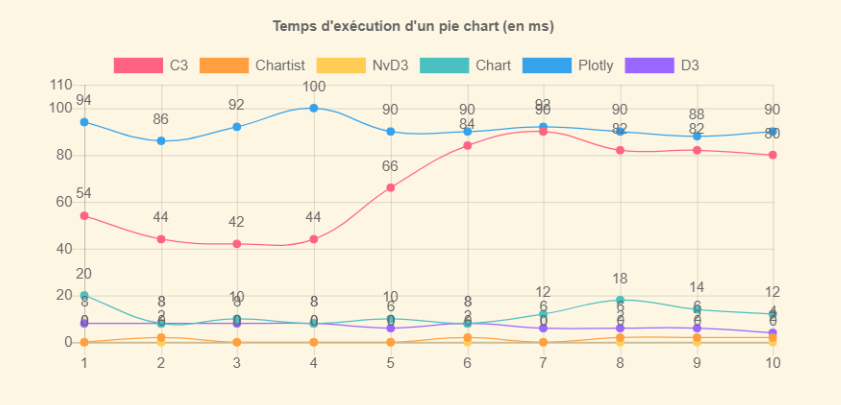
\includegraphics[scale=0.8]{resources/benchmark.png}
\caption{Exemple de l'indicateur "Temps d'exécution" des bibliothèques sur 10 exécutions}
\end{center}
\end{figure}


En plus de ces indicateurs, des critères jugés pertinents ont été rajoutés notamment un critère de notoriété de la bibliothèque. Derrière cela l'idée que si un outil est populaire, cela signifie qu'il y a plus de personnes qui l'utilisent et donc une plus grande communauté pour répondre aux questions, corriger des bogues, etc. Par ailleurs les chiffres disponibles sur les dépôts GitHub ont donc été analysés et plus particulièrement le nombre de téléchargements, de \textit{stars}, de \textit{fork} et de \textit{watch}.\\

Des critères de maintenance des bibliothèques s'ajoutent ensuite. Il est important de savoir si la bibliothèque répond aux \textit{pull requests} et si les \textit{issues} sont traitées. Dans le cas contraire, si un problème apparaît lors du développement, il y a peu de chance de trouver une solution par ces méthodes. Il est tout aussi important d'avoir une idée de combien de \textit{commit} ont été faits et leur fréquence, pour avoir une idée de la grandeur du projet et s'il est encore entretenu.\\

La personnalisation qu'offre les bibliothèques - Titre, légende, \textit{tooltip}, \textit{responsive} ou encore zoom du graphique, la possibilité de personnaliser un graphique - est un avantage et évite d'avoir à tout redéfinir soi-même. Cela économise du temps et évite de potentiels conflits avec la bibliothèque comme la redéfinition de fonctions ou le changement d'éléments du DOM.\\

C'est avec tous ces critères que 6 bibliothèques ont été comparées : C3.js~\cite{c3}, Chartist.js, NVD3, Chart.js, Plotly.js et D3. Parmi elles, C.js3, NVD3 et Plotly.js sont des surcouches de D3 mais n'apportent pas de fonctionnalités de plus que D3, ces bibliothèques permettent juste de produire du code D3 plus rapidement. Par ailleurs, Chartist.js est très limitée en choix de graphiques (3 types : \textit{bar}, \textit{line} et \textit{pie} \textit{charts}) mais a l'avantage d'être très légère (seulement 40 Ko). Enfin Chart.js est la seule à proposer uniquement des graphiques au format Canvas.\\

Après concertation, mon choix s'est porté sur D3. Les plus-values des surcouches D3 n'étaient pas suffisamment importantes pour les retenir. Chartist.js ne proposait pas suffisamment de solutions pour l'outil à développer, il aurait fallu ajouter une autre bibliothèque. Enfin Chart.js était une bonne alternative puisqu'elle proposait des graphiques visuellement intéressants et faciles à construire, néanmoins, le manque d'interaction entre eux et le fait qu'ils soient au format Canvas compliquent l'ajout ou la modification de fonctionnalités.\\


Une fois la bibliothèque choisie, je me suis concentré sur l'utilisation de \textit{Google Analytics}.\\

\subsection{Google Analytics}
\textit{Google Analytics} est un service gratuit qui permet de mesurer l'audience d'un site web. On peut accéder à toutes les données calculées depuis une interface web. Dans un premier temps et afin d'éviter une simple duplication de données, une analyse de ce que propose le service était nécessaire. Cela permettait de définir les informations à croiser avec les données de \textit{finElink}. Une notion importante trouvée fut la possibilité de voir la fréquence de visite d'un dispositif de financement de l'innovation pour chaque utilisateur. Cela permet de créer un coefficient de popularité variable selon une deuxième information, comme la répartition des dispositifs dans un secteur d'activité.\\

Suite à cette analyse, il a fallu apprendre l'utilisation de l'API fournie par Google~\cite{gaapi}. Une problématique de nombre de requêtes par jour, limité à 50 000 par jour, est alors apparue. Dans un contexte de développement, et sûrement après la mise en production, ce palier ne sera jamais atteint. En revanche, il semblait nécessaire de prendre en compte le fait de ne jamais atteindre cette limitation. Si pour une raison quelconque, elle était atteinte, l'intégrité du site en serait impactée pour le reste de la journée. Je me suis donc intéressé à l'utilisation d'un cache dans Django.

\subsection{Cache Django}
Django propose 6 caches différents :
\begin{itemize}
\item \textit{Memcached}, un serveur de cache basé en mémoire.
\item \textit{Database caching} qui stocke les données dans une base de données.
\item \textit{Filesystem caching} enregistre le cache dans des fichiers séparés pour chaque valeur.
\item \textit{Local-memory caching}, cache par défaut de Django, est une alternative au \textit{Memcached}.
\item \textit{Dummy caching} est une implémentation de cache sans action réelle destinée au développement.
\item L'utilisation d'un cache personnalisé.
\end{itemize}
Il était nécessaire d'étudier la performance de chaque cache à l'aide de \textit{benchmarks} et il s'est avéré que le cache par défaut de Django, \textit{local-memory caching} était le plus performant sur les opérations \textit{get}, \textit{set} et \textit{delete}~\cite{CacheBench}. Il semblait donc préférable d'utiliser ce cache pour pallier le nombre limité de requêtes journalières. La durée de ce cache est modifiable dans un fichier de configuration de Django. J'ai proposé d'implémenter une durée d'une journée avant de vider celui-ci. Cela permet d'avoir une mise à jour journalière qui peut être particulièrement intéressante en cas de forte utilisation de \textit{finElink}, comme le cas de l'annonce d'un nouveau dispositif de financement. Une durée plus courte n'est pas nécessaire car les prises de décision, de nature stratégique, pouvant découler de \textit{Business Explorer} ne peuvent pas être faites en temps réel.

\subsection{Visualisation des secteurs d'activité}
La première partie de la réalisation graphique de la datavisualisation s'est portée sur les secteurs d'activités des dispositifs de financement de l'innovation. Pour chaque secteur, les données à valoriser était : 
\begin{itemize}
\item la popularité,
\item le budget alloué,
\item le nombre de dispositifs,
\item la répartition géographique (si c'est un dispositif régional, européen, etc.),
\item la collaboration est-elle obligatoire ?
\end{itemize}
Ces informations semblaient être les plus pertinentes à mettre en exergue pour avoir un aperçu des tendances, de l'importance donnée à un secteur d'activité. Par exemple si le secteur de l'environnement dispose du budget de financement le plus conséquent alors que les dispositifs finançant les secteurs informatiques ou de technologies de pointe sont les plus sollicités. Pour éviter l'afflux d'informations, il semblait important d'épurer et donc se recentrer sur l'essentiel, c'est-à-dire la popularité, le budget alloué et le nombre de dispositifs. Cette étape a nécessité une grande réflexion car il fallait identifier les indicateurs les plus importants tout en respectant l'esthétique de la page.\\

Dans un premier temps, les données de \textit{Google Analytics} sont récupérées, suivies de celles de \textit{finElink}. Ces deux jeux de données (\textit{datasets}) sont ensuite envoyés à une fonction qui s'occupera de les mettre en commun (figure 5.2). Le \textit{dataset} obtenu est ensuite envoyé au template Django pour être affiché. 

\begin{figure}
\begin{center}
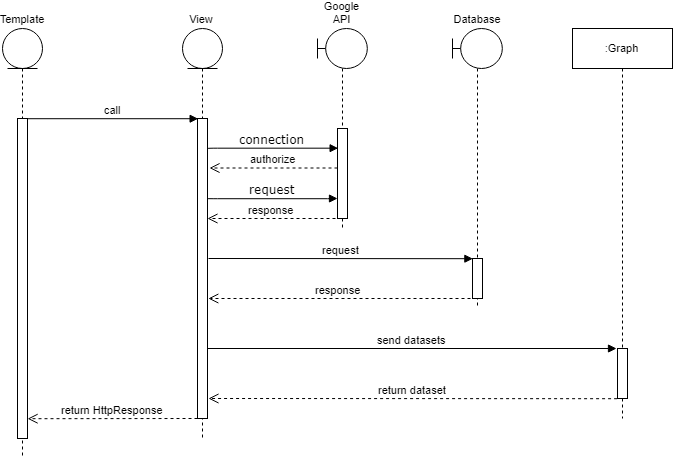
\includegraphics[scale=0.65]{resources/sequence_diagram_chart.png}
\caption{Fonctionnement d'un traitement de données de \textit{Business Explorer}}
\end{center}
\end{figure}

Une fois le choix des indicateurs fait, le camembert semblait initalement intéressant. Cependant, cela s'est avéré difficile de faire des comparaisons à partir de ce type de graphique. Par la suite, un \textit{sunburst chart} s'avéra plus pertinent pour représenter l'ensemble des informations et pouvoir ainsi mieux les comparer. La répartition de chaque secteur ainsi que l'animation faite lors du changement d'indicateur a permis de représenter dans un graphique chaque secteur, son indicateur et la possibilité de comparer avec l'ensemble des indicateurs (figure 5.3).\\

\begin{figure}
\begin{center}
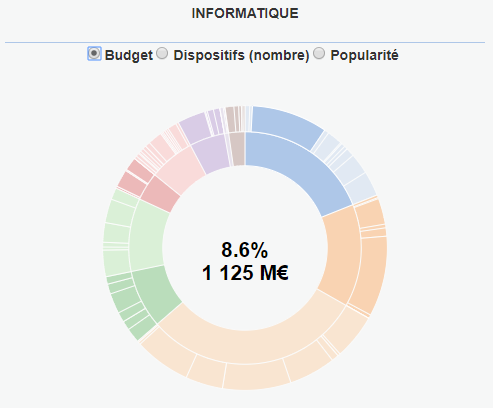
\includegraphics[scale=1]{resources/sunburst.png}
\caption{Sunburst présentant le budget alloué pour les projets informatiques}
\end{center}
\end{figure}

Ensuite, pour assurer l'interaction dans le \textit{sunburst chart}, il a été ajouté un tableau de données et un histogramme permettant de positionner une thématique dans son secteur et le secteur dans son ensemble pour affiner les informations qui étaient déjà présentes.